
% ********** Chapter 11 **********
\chapter{Conclusion}
\label{sec:Conclusion}

\lettrine[lines=3]{T}{his} dissertation has focused on the solution and implementation of Web Call Example Application. In the solution part, it introduces the theory of manipulating SIP message to achieve third party call control. And in implementation part, it covers all the components of Web Call Example Application.

\section{Conclusion of solution}

Two kind of connection solution of the core of Web Call are introduced, they are Relay Call and Third Party Call. This article explained the drawback of Relay Call and how third party call could cover these facts. Four different implementations of third party call are introduced in detail with SIP message flow.

\textsf{Relay Call} is the legacy solution of previous version of \textsf{Web Call Example Application}. According to \textit{Web Call SDK} \cite{WebCallSDK}, the \textsf{Relay Call} controller works as an User Agent Client, connect two sessions and transfer media flow from one session to another. It can be used in any standard SIP network with the drawback of relevant long latency and long connection time.

\textsf{Call Transfer} is a solution of third party call that uses \textit{The Session Initiation Protocol (SIP) Refer Method (RFC 3515)} \cite{RFC3515}. When connect with the Client A, controller sends a \texttt{REFER} signal which force Client A calls Client B. This solution needs a support of RFC 3515 at client side.

\textsf{SDP Swap} is a solution of third party call that manipulates SIP messages. While the hand shake with Client A and Client B, controller swaps SDP message from A and B. This makes Client A and Client B's media flow go direct to each other.  It is a very efficient solution with limitation. SIP message without SDP will be used in this solution. Though it is validate according to \textit{SIP: Session Initiation Protocol 
(RFC 3261)} \cite{RFC3261}, some service provider may treat such kind of message as illegal. 

\textsf{Re-invite} is a solution of third party call that use a \texttt{RE-INVITE} message to re-establish media flow. At the first phase of hand shake, controller collects SDP from Client A and Client B. At the second phase, controller swaps the SDPs via a \texttt{RE-INVITE} to Client A and Client B. It is also a very efficient solution with limitation. \texttt{RE-INVITE} message will be treated as invalid message by some service provider.

\textsf{Web Client} is a solution of third party call that works as a HTTP client to communicate with the provider's web portal. It does not manipulate any SIP message at all. Instead, it send HTTP request to the web site, and the VoIP connection will be established by the native method of VoIP service provider.

\section{Conclusion of application}

Web Call Example Application is an application that hosted by a web server and supplies functionality of VoIP phone calls. The thesis covered all components of the application. \textsf{SIP Call Component}, \textsf{Web Application}, \textsf{Web Service Interface} and \textsf{Java ME client} are all introduced in the article. 

\textsf{SIP call component} is a high level API that used for making VoIP phone calls. It integrated five different methods. It is the core stack of \textsf{Web Call Example Application}. It is designed to work as a standalone library and can be used in other applications. The abstract factory in SIP call component gives a very convenient way to initialize different call controllers.

\textsf{Web Application} is a component that supplies variety functions of VoIP call, and furthermore, it supplies a way of managing SIP account and contact books. Based on Mobile Front Controller, Web Application provides two view that is desktop browser view and mobile browser view. The two views are special optimized for different type of web browsers.

\textsf{Web Service interface} is a common interface of Web Call Example Application. It bases on SOAP Web Service technology, implements most of the functions of Web Application. Besides that, it also contains a feature of synchronize contact book. Java ME client is one of the possible clients of Web Service interface.

\textsf{Java ME client} is a client of Web Service interface. The main purpose of it is to give a way of fast dial. It can record all the latest operations include the number of caller and callee. The last used call method will also be stored in the Java ME client. It can also load the native contact book of mobile phone and store it into contact book of Web Application.


\section{Future Work}
\label{sec:Conclusion:FutureWork}

There are many other tasks can be counted into requirements of Web Call Example Application. For the limitation of time and resources, they are planned to be implemented in the next version of release.

\subsection{Switch SIP stack to JSR 32}

Most of our implementations are based on MjSIP, which is already stopped maintenance in year 2006. \cite{MjSip} So it is not a good idea to continue working with this SIP stack. 

JSR 32 JAIN\texttrademark{} SIP API is the best candidate for base SIP stack. \textit{``The JAIN\texttrademark{} SIP API specification provides a standard portable interface to share information between SIP Clients and SIP Servers, providing call control elements enabling converged-network applications.''} \cite{JSR32} It is a java standard and can be use for free. And furthermore, it is still been well maintained. The latest version is 1.2.

Thanks to the five layers architecture, it will not be a tough work to switch SIP stack API.

\subsection{RESTful web service interface}
\label{sec:Conclusion:FutureWork:RESTfulWebServiceInterface}

Though Web Call Example Application already has a web service as described in chapter \ref{sec:WebServiceInterface}, it cannot be used for all kinds of clients. Current web service interface in Web Call Example Application is based on SOAP. The SOAP based Java ME Client requires a JSR 172 supported device. However, not all the devices are designed to have such API. e.g., most windows mobile based cell phones do not supply JSR 172. On the other side, almost all mobile phones have a HTTP connection support. And it is enough to have a RESTful web service client. RESTful web service can also be used for web 2.0 mushup.

There is an application called \textsf{RESTful Web Call Gateway} which is developed by \textit{Peter Yeung} from Ericsson Developer Connection. It is a RESTful web service gateway based on Web Call Example Application. It is like a gateway convert SOAP web service to RESTful web service. The architecture of RESTful Web Call Gateway and use case is shown in Figure \ref{fig:RESTWebCallGateway}.

However, the RESTful Web Call Gateway is not a native interface of Web Call Example Application. So it is not that efficiency. A good design should be that have both SOAP web service and RESTful web service on top of SIP Call Component.

\begin{sidewaysfigure}[!hbtp]
\centering
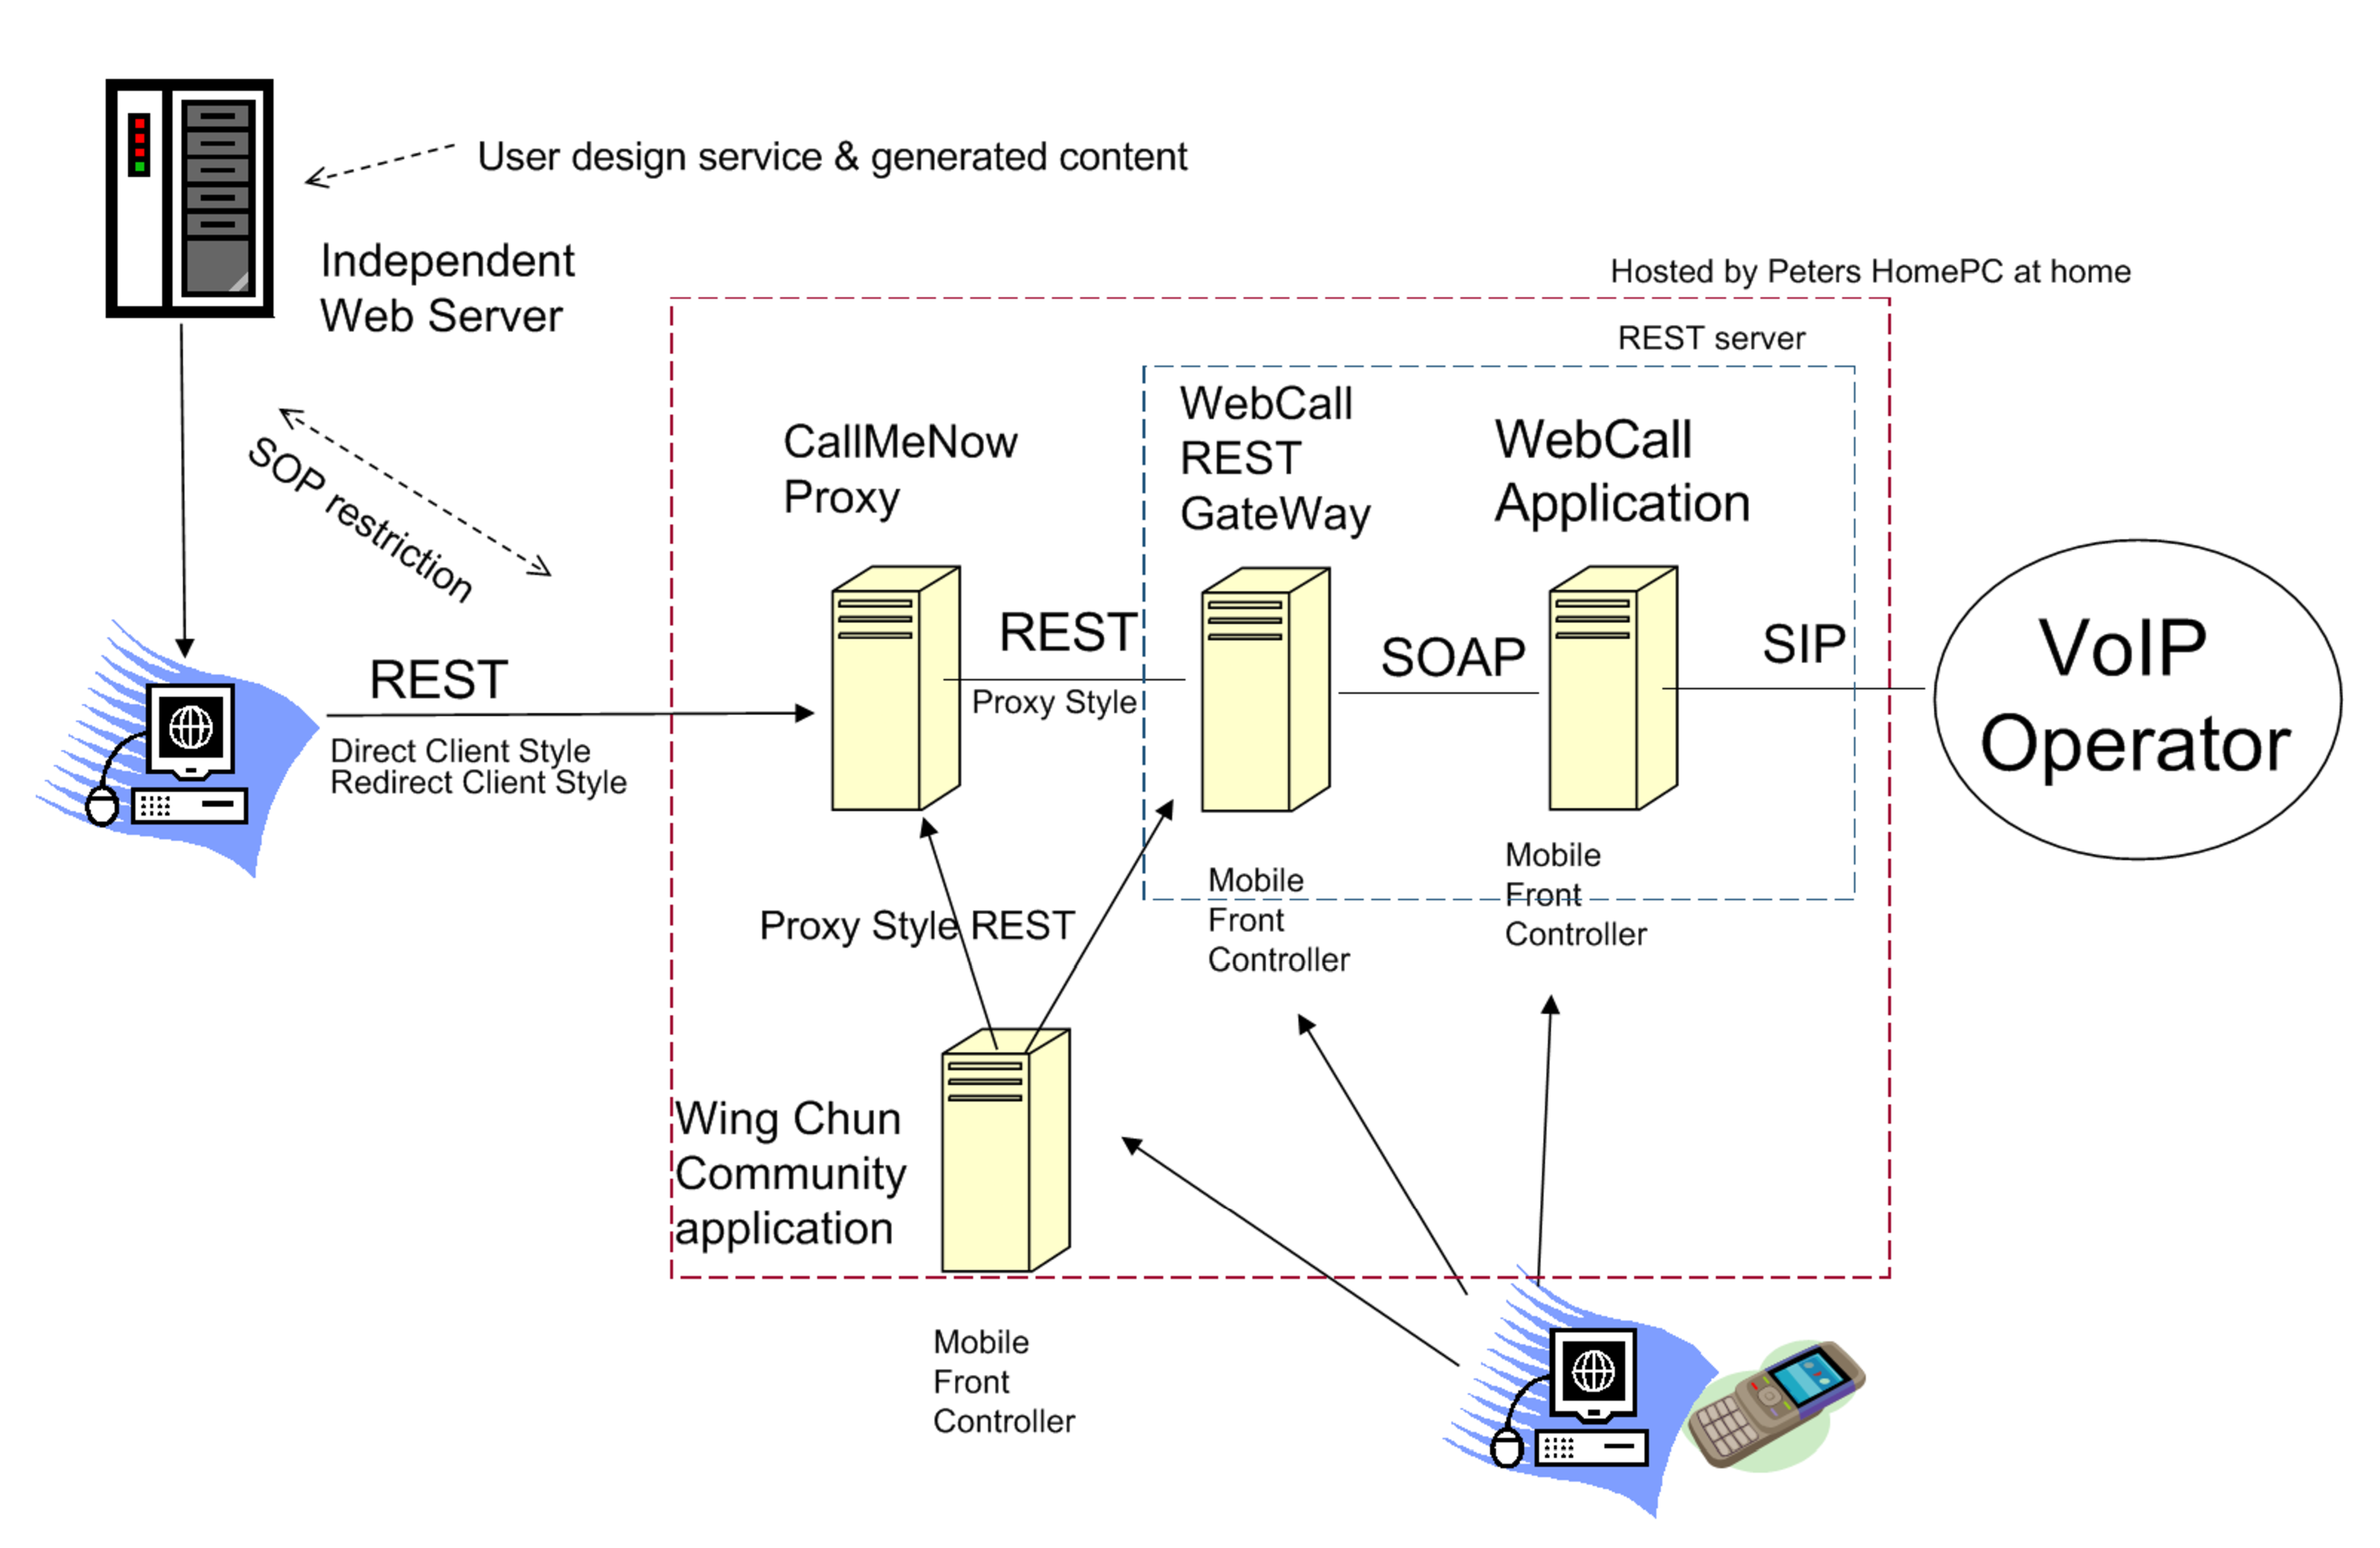
\epsfig{file=chap10/resources/REST_webcall_gateway, width=8.3in}
\caption{REST web call gateway (Figure taken from \textit{Using REST and Web Services to Mash Up Communications Capabilities} by Elena Fersman and Peter Yeung \cite{DemoAtJavaOne})}
\label{fig:RESTWebCallGateway}
\end{sidewaysfigure}

\subsection{Gadgets}
\label{sec:Conclusion:FutureWork:Gadgets}

There could be many gadgets client for Web Call Example Application. Most of them will use RESTful web service interface. The gadgets could be Facebook gadget, igoogle gadget, or Vista sidebar gadget. A vista gadget \textsf{Call You Now} was developed by Peter Yeung. It uses the RESTful web service supplied by RESTful Web Call Gateway.

\subsection{Call history}
\label{sec:Conclusion:FutureWork:CallHistory}

If an administrator wants to know the call histories, the only way is to see the server log. However, it is not convenient. And it is also hard to manage the call logs. There is also a plan for next release of web call to add call histories to database. So it is easy to track and manage.

% ********** End of chapter **********
